\documentclass{article}

\usepackage[english]{babel}
\usepackage[utf8]{inputenc}
\usepackage[document]{ragged2e}
\usepackage{lipsum}% Just for this example
\usepackage{graphicx}
\usepackage{amsmath,amssymb}

\usepackage{parskip}
\usepackage{graphicx}

% Margins
\usepackage[top=2.5cm, left=3cm, right=3cm, bottom=4.0cm]{geometry}
% Colour table cells
\usepackage[table]{xcolor}

% Get larger line spacing in table
\newcommand{\tablespace}{\\[1.25mm]}
\newcommand\Tstrut{\rule{0pt}{2.6ex}}         % = `top' strut
\newcommand\tstrut{\rule{0pt}{2.0ex}}         % = `top' strut
\newcommand\Bstrut{\rule[-0.9ex]{0pt}{0pt}}   % = `bottom' strut

%%%%%%%%%%%%%%%%%
%     Title     %
%%%%%%%%%%%%%%%%%
\title{Introduction to Econometrics: Assignment 1}
\author{Yanis Ferhat (11288574) \and Félix Poirier (11298801) \and Joel Chrispin (11288382)}
\usepackage{datetime}
\newdate{date}{29}{09}{2022}
\date{\displaydate{date}}

\begin{document}
\maketitle

%%%%%%%%%%%%%%%%%
%   Problem 1   %
%%%%%%%%%%%%%%%%%
\section{Question 1}
Our research question is the following: Can changes in US business activity and confidence be affected by changes in China’s business conditions 3 months earlier? In other words, we are analyzing whether changes in China business conditions can be a good forward indicator for changes in US business conditions. This question is of interest notably because of the pandemic which has shown how central China's industries are to the global economy. Within the confines of this assignment we will explore if China's business activity and confidence has a relationship to business activity and confidence in its biggest economic partner, the United States. Some believe that downturns in China’s economy usually precede the Western world’s downturns by a few months, within the context of this research we've chosen to analyze the relationship in-between three months (a quarter). This research question will allow us to analyze the strength of the relationship between the United State's PMI and China's PMI from 3 months ago. We will be using both countries’ monthly PMI indicators to measure business activity and confidence. We expect to see no relationship as the economy tends to be efficient between nations, in which case the random walks theory would suggest that past information has no say on future outcomes.

%%%%%%%%%%%%%%%%%
%   Problem 2   %
%%%%%%%%%%%%%%%%%
\section{Question 2}
\textit{Data source: Bloomberg, 2022, “NAPMPMI” \& “CPMINDX” (accessed September 8th, 2022)}

The data set we used for this assignment was constructed manually from two tables that were extracted from Bloomberg. The first table is a time series detailing the US PMI monthly indicator from April 30th, 2016, to August 31st, 2022. The second table is a time series of the China PMI monthly indicator from January 1st, 2016, to May 31st, 2022. PMI stands for Purchasing Managers’ Index and is “an index of the prevailing direction of economic trends in the manufacturing and service sectors. It consists of a diffusion index that summarizes whether market conditions, as viewed by purchasing managers, are expanding, staying the same, or contracting. The purpose of the PMI is to provide information about current and future business conditions to company decision makers, analysts, and investors.” (Investopedia, 2022). Both tables show the value of the indicator for every included month, its net change from month to month as well as its percent change. The latter is the information we used to create our final dataset. Therefore, the final dataset consists of two variables. The first represents the percent change in the US PMI indicator, which we declared as $\textbf{uspchange}$. The second, denoted $\textbf{chipchange}$, represents the percent change in the China PMI indicator recorded 3 months earlier than its american equivalent.

%%%%%%%%%%%%%%%%%
%   Problem 3   %
%%%%%%%%%%%%%%%%%
\section{Question 3}

Below is a table of summary statistics describing the variables that were of interest in our analysis.
\begin{center}

\title{Table 1: Descriptibe statistics for uspchange and chipchange}

\begin{tabular}{lrr}
{} &  \textbf{} &  chipchange \\
count &  76.000000 &   76.000000 \\
mean  &   0.001166 &    0.001860 \\
std   &   0.040315 &    0.063457 \\
min   &  -0.152749 &   -0.286000 \\
25\%   &  -0.020505 &   -0.007957 \\
50\%   &   0.000000 &   -0.001959 \\
75\%   &   0.018660 &    0.005868 \\
max   &   0.204598 &    0.456583 \\
\end{tabular}

\textit{Table from pandas' DataFrame .describe() method}

\end{center}


The mean values for uspchange and chipchange are 0.117\% and 0.186\%, respectively. This indicates that, on average, the monthly percent change in the US and China PMI indicators during their respective time periods were 0.117 \% and 0.186 \%, respectively. The standard deviation for uspchange is 4.032 \%, which indicates that the average difference between a month’s PMI percent change and the mean percent change is 4.032\%. The standard deviation for chipchange is 6.346 \%, meaning the average difference between a month’s PMI percent change and the average percent change is 6.346 \%. US PMI variations ranged from -15.275 \% to 20.460 \%. China PMI variations ranged from -28.6 \% to 45.658 \%. In brief, this group of descriptive statistics shows that the dispersion in chipchange’s range of values is much larger than uspchange’s. 

\begin{table}
\begin{figure}
  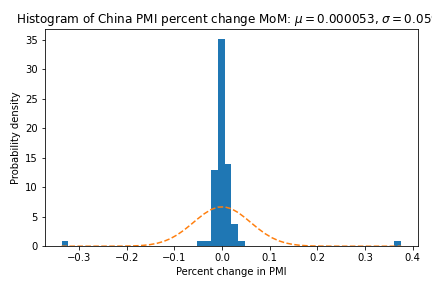
\includegraphics[width=\linewidth]{/images/distribution_China_PMI.png}
  \caption{A boat.}
  \label{fig:boat1}
\end{figure}
\end{table}







%%%%%%%%%%%%%%%%%
%   Problem 3   %
%%%%%%%%%%%%%%%%%
\section{Question 4}

The equation below is the econometric model at the forefront of our analysis.

\begin{center}
$uspchange_i = \beta_0 + \beta_1 chipchange_i + u_i $\end{center}
Using the \emph{OLS} function from Python's \emph{statsmodels} package, we were able to estimate the above theoretical model. Here is a table detailing the estimation's results:





\end{document}
